% Digital Logic Report Template
% Created: 2020-01-10, John Miller

%==========================================================
%=========== Document Setup  ==============================

% Formatting defined by class file
\documentclass[11pt]{article}

% ---- Document formatting ----
\usepackage[margin=1in]{geometry}	% Narrower margins
\usepackage{booktabs}				% Nice formatting of tables
\usepackage{graphicx}				% Ability to include graphics

%\setlength\parindent{0pt}	% Do not indent first line of paragraphs 
\usepackage[parfill]{parskip}		% Line space b/w paragraphs
%	parfill option prevents last line of pgrph from being fully justified

% Parskip package adds too much space around titles, fix with this
\RequirePackage{titlesec}
\titlespacing\section{0pt}{8pt plus 4pt minus 2pt}{3pt plus 2pt minus 2pt}
\titlespacing\subsection{0pt}{4pt plus 4pt minus 2pt}{-2pt plus 2pt minus 2pt}
\titlespacing\subsubsection{0pt}{2pt plus 4pt minus 2pt}{-6pt plus 2pt minus 2pt}

% ---- Hyperlinks ----
\usepackage[colorlinks=true,urlcolor=blue]{hyperref}	% For URL's. Automatically links internal references.

% ---- Code listings ----
\usepackage{listings} 					% Nice code layout and inclusion
\usepackage[usenames,dvipsnames]{xcolor}	% Colors (needs to be defined before using colors)

% Define custom colors for listings
\definecolor{listinggray}{gray}{0.98}		% Listings background color
\definecolor{rulegray}{gray}{0.7}			% Listings rule/frame color

% Style for Verilog
\lstdefinestyle{Verilog}{
	language=Verilog,					% Verilog
	backgroundcolor=\color{listinggray},	% light gray background
	rulecolor=\color{blue}, 			% blue frame lines
	frame=tb,							% lines above & below
	linewidth=\columnwidth, 			% set line width
	basicstyle=\small\ttfamily,	% basic font style that is used for the code	
	breaklines=true, 					% allow breaking across columns/pages
	tabsize=3,							% set tab size
	commentstyle=\color{gray},	% comments in italic 
	stringstyle=\upshape,				% strings are printed in normal font
	showspaces=false,					% don't underscore spaces
}

% How to use: \Verilog[listing_options]{file}
\newcommand{\Verilog}[2][]{%
	\lstinputlisting[style=Verilog,#1]{#2}
}




%======================================================
%=========== Body  ====================================
\begin{document}

\title{ELC 2137 Lab 10: 7-segment Display with Time-Division Multiplexing}
\author{Jake Simmons}

\maketitle


\section*{Summary}

The purpose of this lab was to learn how to use the technique called Time-Division Multiplexing. We are using Time-Division Multiplexing to slow down the signals going to the 4 digit display. This is so there will be enough time for a human to process and see what is actually being displayed. First, a counter module was made and succesfully simulated. Secondly, the sseg4 from a previous lab was modified and the counter was added to the module. A schematic of the new, sseg4TDM, is provided. After testing sseg4TDM, the top level module, calclab10, was created. The top level module toplab9 was used in this module which was also created in a previous lab.  

\clearpage
\section*{Q\&A}

\begin{enumerate}
		\item What are the three main “groups” of the RTL definition of sequential logic?
		\begin{enumerate}
			\item 	The three main groups of the RTL definitions of sequential logic is event driven, clock driven and pulse driven. 
		\end{enumerate}
	
	\item Copy Figure 10.3b onto your own paper (or do it electronically) and draw three boxes around the components that belong to each group. Include your annotated figure in your report.
	
	\begin{figure}[ht]\centering
		\caption{10.3B Labeling}
	%	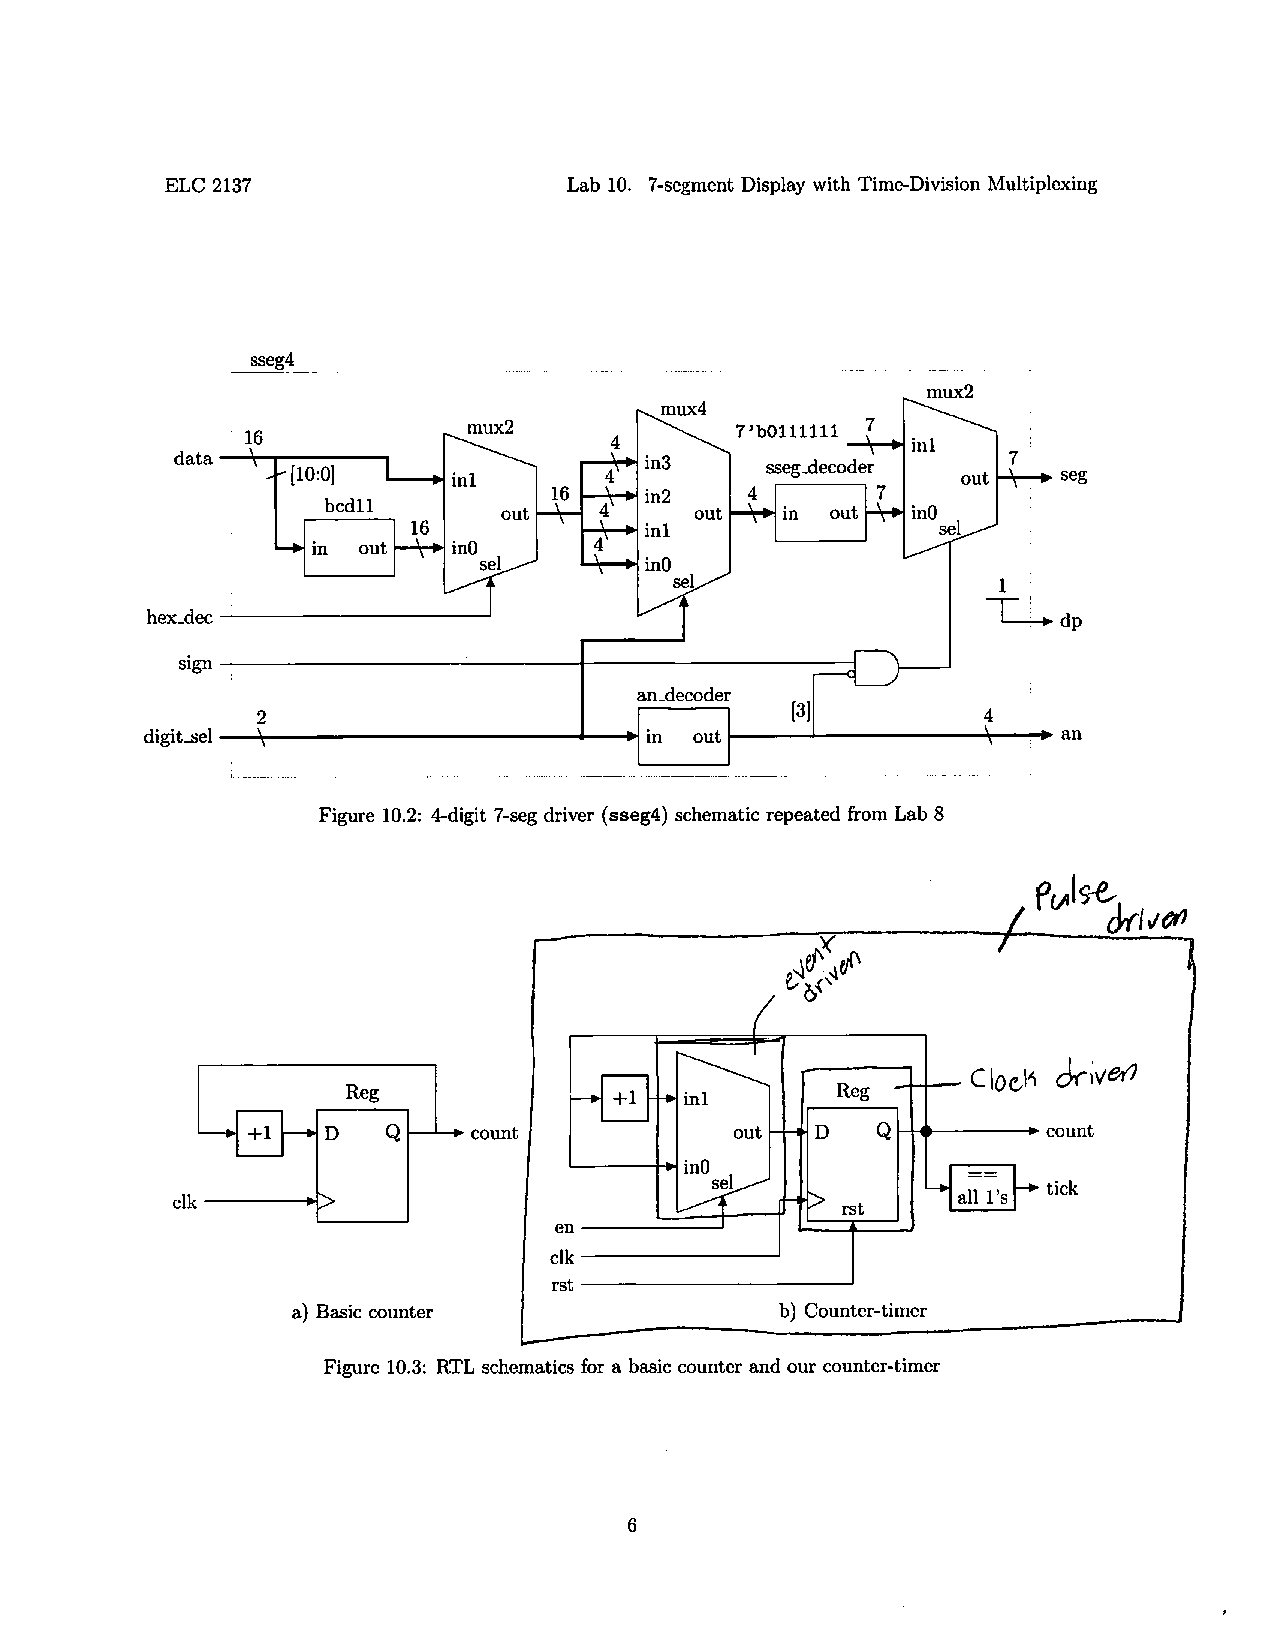
\includegraphics[trim={8.8cm 5cm 0cm 14cm},clip]{10.3_b.pdf}
		\label{fig:picture}
	\end{figure}

	\item If instead of a counter, you wanted to make a shift register that moved the input bits from right to left (low to high). What would you put on the line Q next = /*???*/
	\begin{enumerate}
		\item To make a shift register that moved bits from right to left, you would put on the line Q next = Q reg - 1;
	\end{enumerate}
\end{enumerate}


\clearpage
\section*{Results}

\begin{figure}[ht]\centering
	\begin{tabular}{l|rrrrrrrrrrrrrrrr}
		Time (ns): & 0 & 50 & 100 & 150 & 200  & 250 & 300 & 350 & 400 & 450 & 500 & 550 & 600 & 650 & 700  & 750\\
		\midrule
		clk & 0 & 1 & 1 & 1 & 1 & 1 & 1 & 1 & 1 & 1 & 1 & 1 & 1 & 1 & 1 & 1\\
		rst & 1 & 0 & 0 & 0 & 0 & 0 & 0 & 0 & 0 & 0 & 0 & 0 & 0 & 0 & 0 & 0 \\
		in & 0 & 1 & 1 & 0 & 1 & 1 & 1 & 1 & 1 & 0 & 1 & 1 & 1 & 0 & 0 & 0 \\
		\midrule
		out & X & 0 & 0 & 0 & 0 & 1 & 1 & 1 & 1 & 1 & 1 & 1 & 1 & 0 & 0 & 0 \\
		tick & X & 0 & 0 & 0 & 0 & 1 & 0 & 0 & 0 & 0 & 0 & 0 & 0 & 0 & 0 & 0 \\
		i & X & 0 & 1 & 4 & 6 & 9 & a & a & a & a & 1 & 4 & 6 & 9 & a & a \\
		\bottomrule
	\end{tabular}\medskip
	
	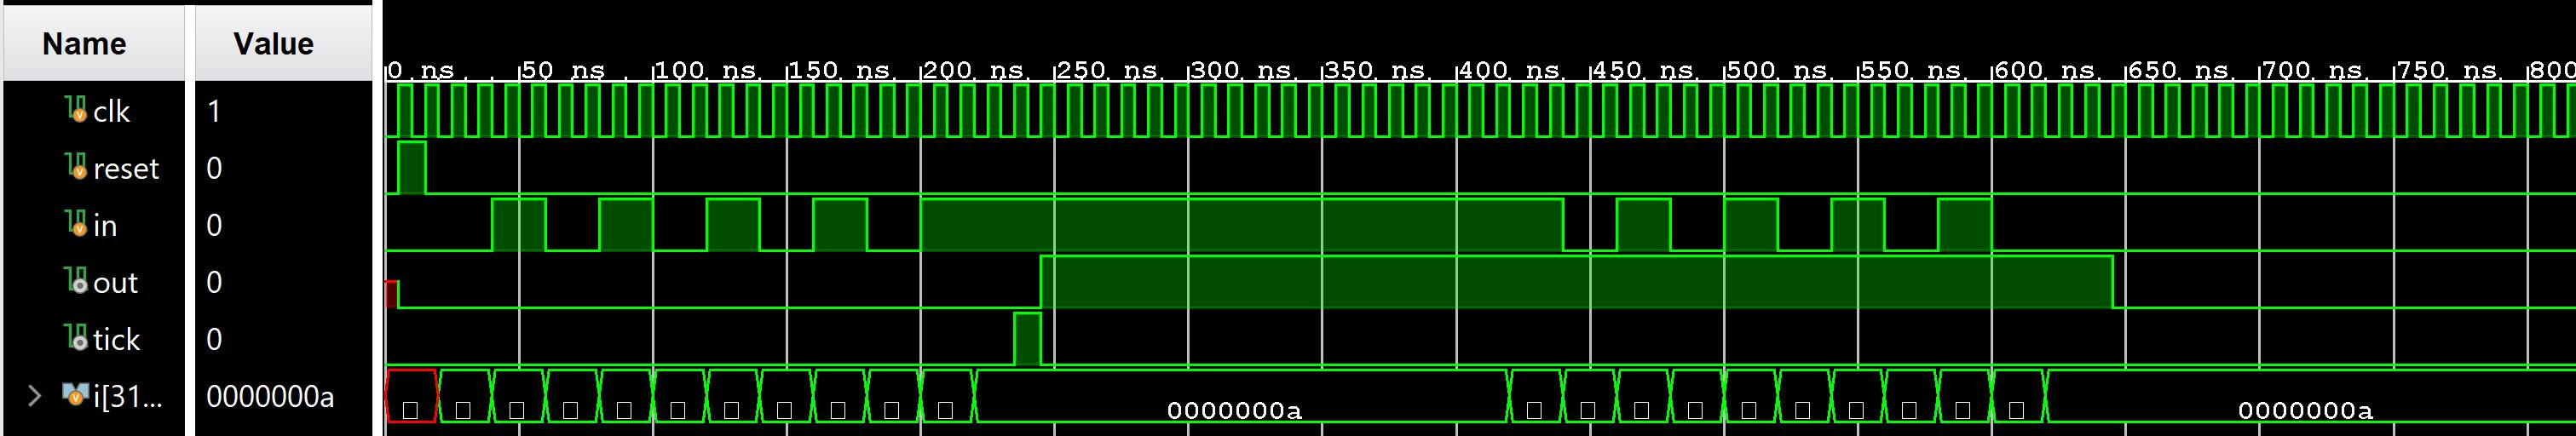
\includegraphics[trim=0cm 0cm 11cm 0cm, clip]{debounce_test.JPG}
	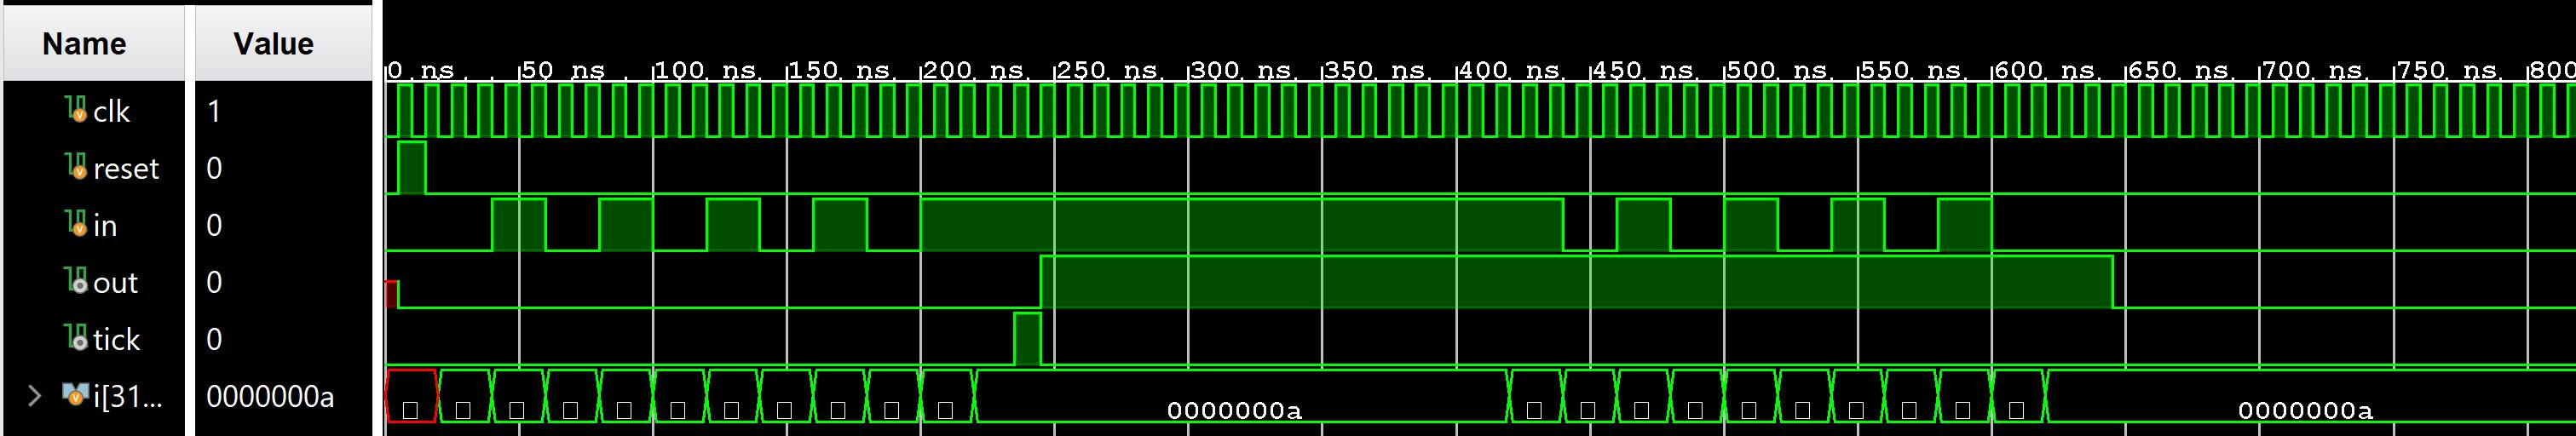
\includegraphics[trim=15cm 0cm 2cm 0cm, clip]{debounce_test.JPG}
	\caption{debounce simulation waveform and ERT}
	\label{fig:sim_with_table}
\end{figure}

\begin{figure}[ht]\centering
	\begin{tabular}{l|rrrrrrrrrrrrrrrrr}
		Time (ms): & 0 & 25 & 50 & 75 & 100  & 125 & 150 & 175 & 200 & 225 & 250 & 275 & 300 & 325 & 350  & 375 & 400  \\
		\midrule
		clk & 0 & 1 & 1 & 1 & 1 & 1 & 1 & 1 & 1 & 1 & 1 & 1 & 1 & 1 & 1 & 1 & 1\\
		rst & 1 & 0 & 0 & 0 & 0 & 0 & 0 & 0 & 0 & 0 & 0 & 0 & 0 & 0 & 0 & 0 & 0 \\
		b & 0 & 0 & 0 & 1 & 2 & 1 & 0 & 0 & 1 & 0 & 4 & 0 & 1 & 8 & b & 0 & 0 \\
		\midrule
		y & X & 1 & 2 & 4 & 8 & 8 & 1 & 1 & 1 & 1 & 2 & 2 & 1 & 1 & 2 & 2 & 1 \\
		win & X & 0 & 0 & 0 & 0 & 0 & 0 & 0 & 1 & 0 & 1 & 0 & 1 & 0 & 0 & 0 & 0 \\
		lose & X & 0 & 0 & 1 & 0 & 0 & 1 & 0 & 0 & 0 & 0 & 0 & 0 & 0 & 1 & 0 & 1\\
		\bottomrule
	\end{tabular}\medskip

	
	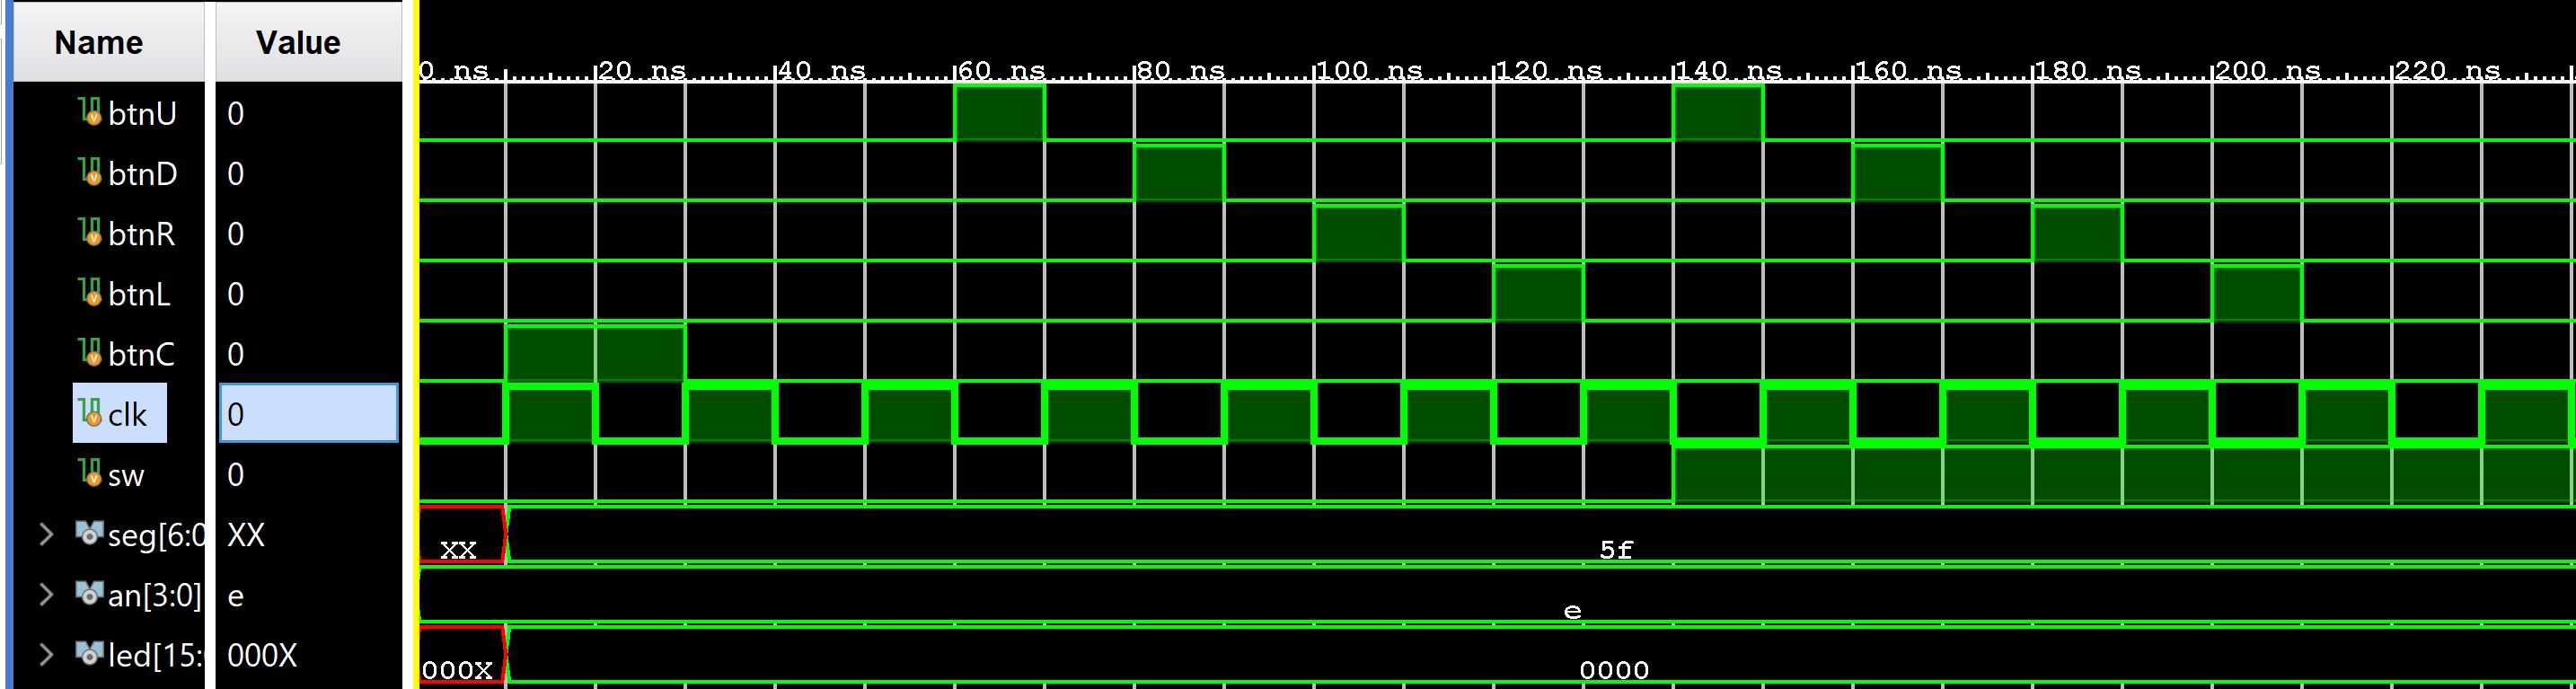
\includegraphics[trim= 0cm 0cm 8cm 0cm]{guess_FSM_test.JPG}

	\caption{guess FSM simulation waveform and ERT}
	\label{fig:sim_with_table}
\end{figure}

\begin{figure}[ht]\centering
	\begin{tabular}{l|rrrrrrrrrrrr}
		Time (ms): & 0 & 20 & 40 & 60 & 80  & 100 & 120 & 140 & 160 & 180 & 200 & 220 \\
		\midrule
		btnU & 0 & 0 & 0 & 1 & 0 & 0 & 0 & 1 & 0 & 0 & 0 & 0  \\
		btnD & 0 & 0 & 0 & 0 & 1 & 0 & 0 & 0 & 1 & 0 & 0 & 0  \\
		btnR & 0 & 0 & 0 & 0 & 0 & 1 & 0 & 0 & 0 & 1 & 0 & 0  \\
		btnL & 0 & 0 & 0 & 0 & 0 & 0 & 1 & 0 & 0 & 0 & 1 & 0  \\
		btnC & 0 & 1 & 0 & 0 & 0 & 0 & 0 & 0 & 0 & 0 & 0 & 0  \\
		clk & 1 & 1 & 1 & 1 & 1 & 1 & 1 & 1 & 1 & 1 & 1 & 1  \\
		sw & 0 & 0 & 0 & 0 & 0 & 0 & 0 & 1 & 1 & 1 & 1 & 1  \\
		\midrule
		seg & X & 5f & 5f & 5f & 5f & 5f & 5f & 5f & 5f & 5f & 5f & 5f  \\
		an & e & e & e & e & e & e & e & e & e & e & e & e  \\
		led & X & 0 & 0 & 0 & 0 & 0 & 0 & 0 & 0 & 0 & 0 & 0  \\
		\midule
	
		\midrule
		
		\bottomrule
	\end{tabular}\medskip
	
	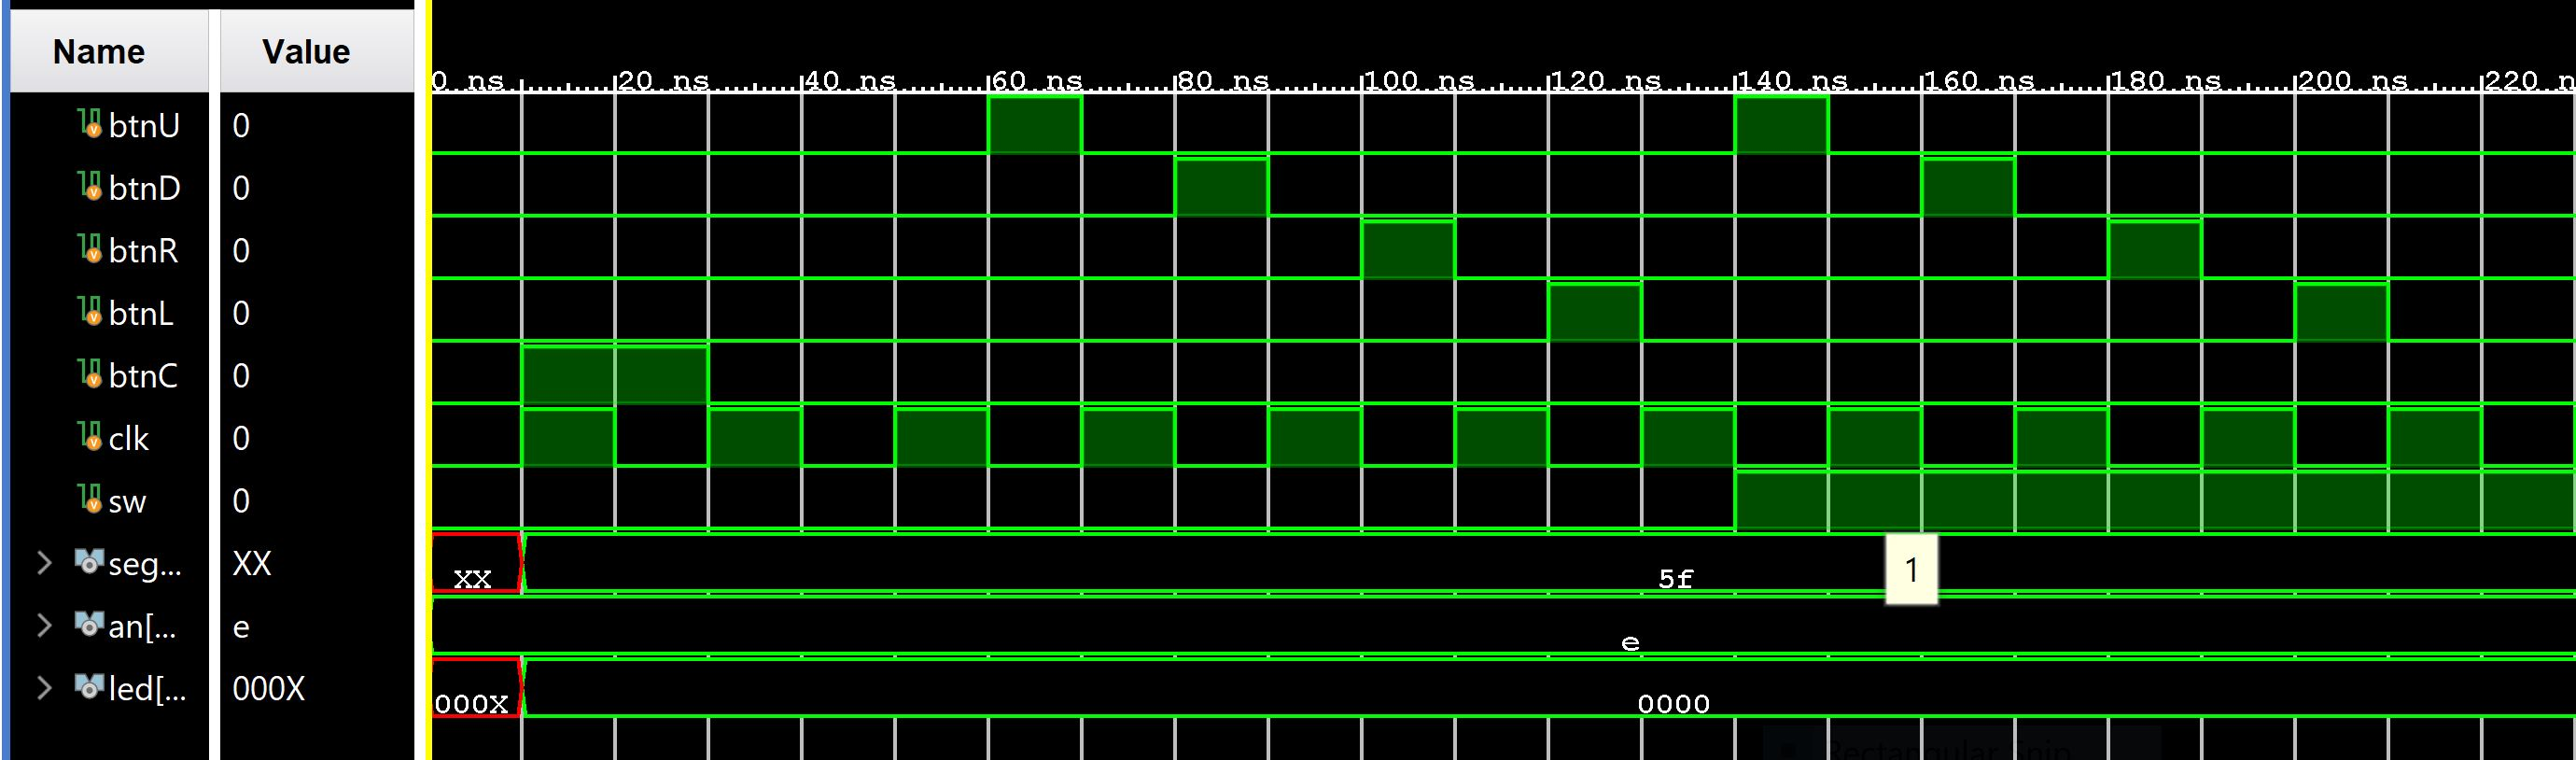
\includegraphics[trim=0cm 0cm 9cm 0cm,clip]{guessing_game_test.JPG}
	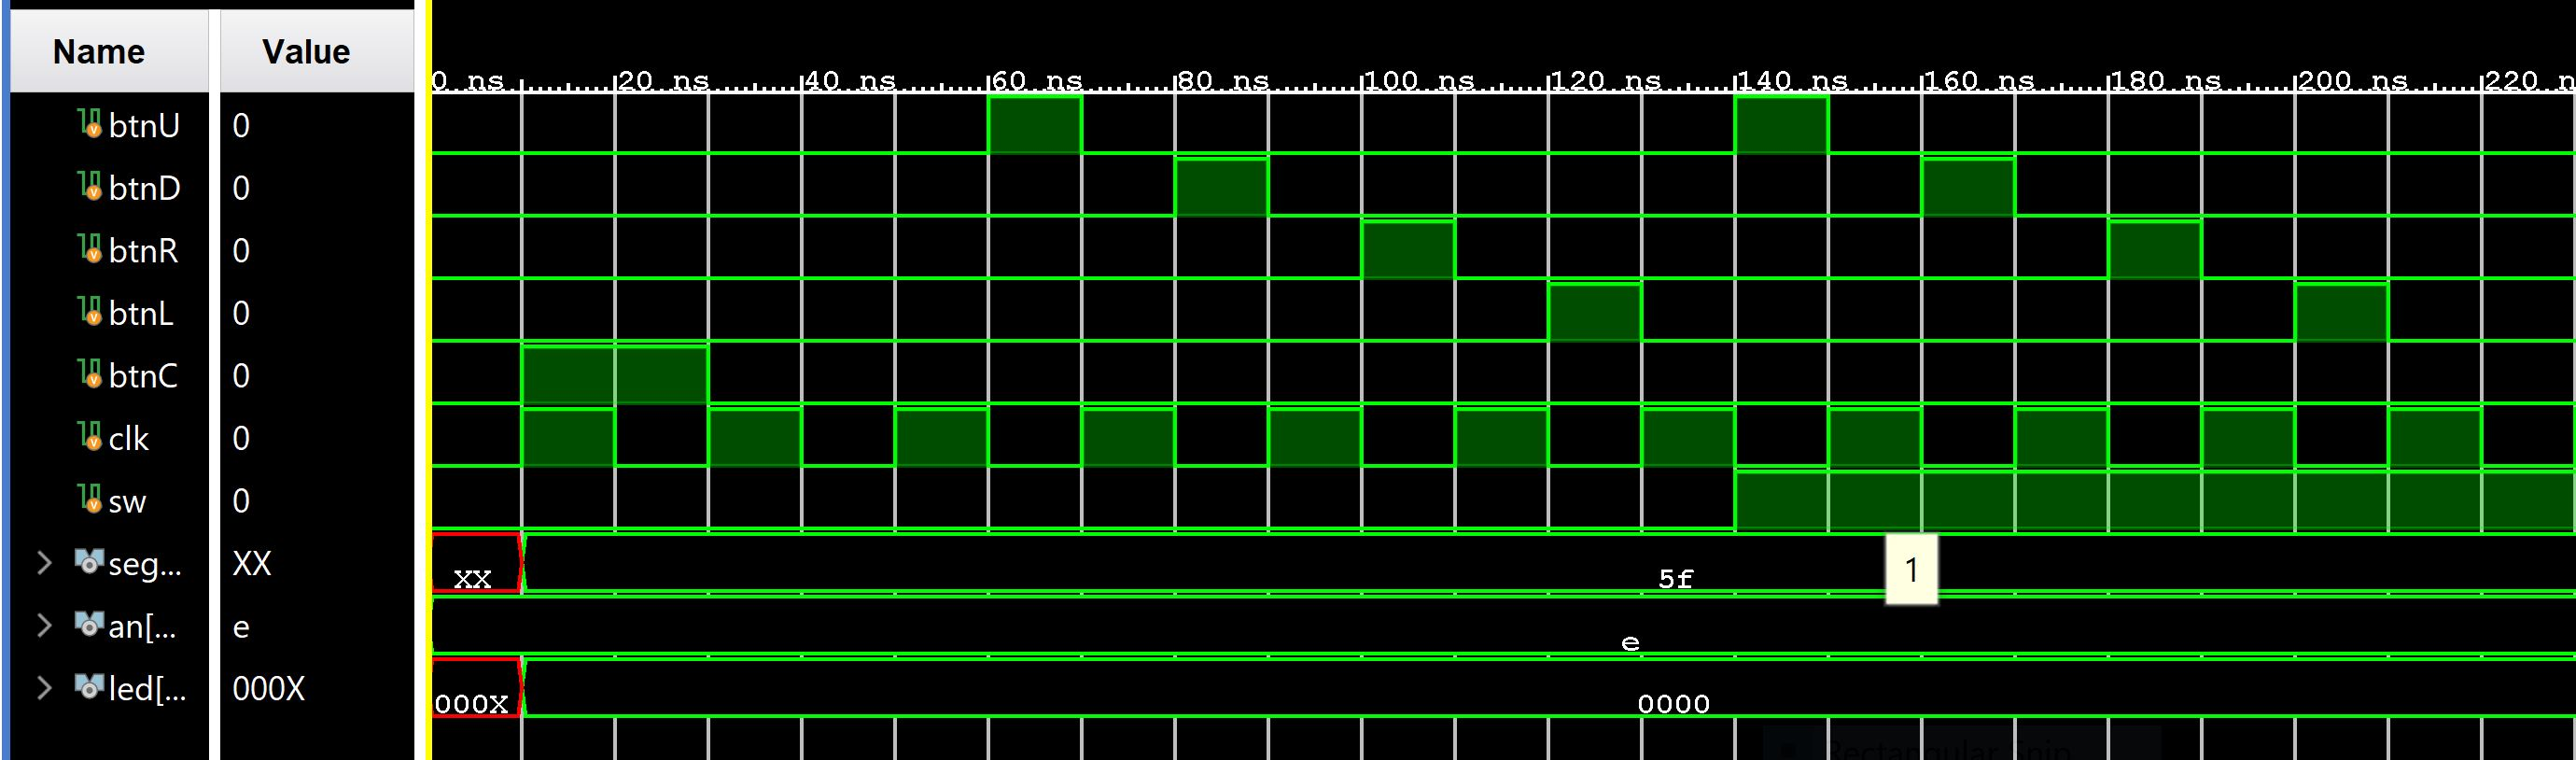
\includegraphics[trim=14.5cm 0cm 0cm 0cm,clip]{guessing_game_test.JPG}
	
	\caption{guess FSM simulation waveform and ERT}
	\label{fig:sim_with_table}
\end{figure}

\begin{figure}[ht]\centering
	\caption{sseg4TDM Schematic}
%	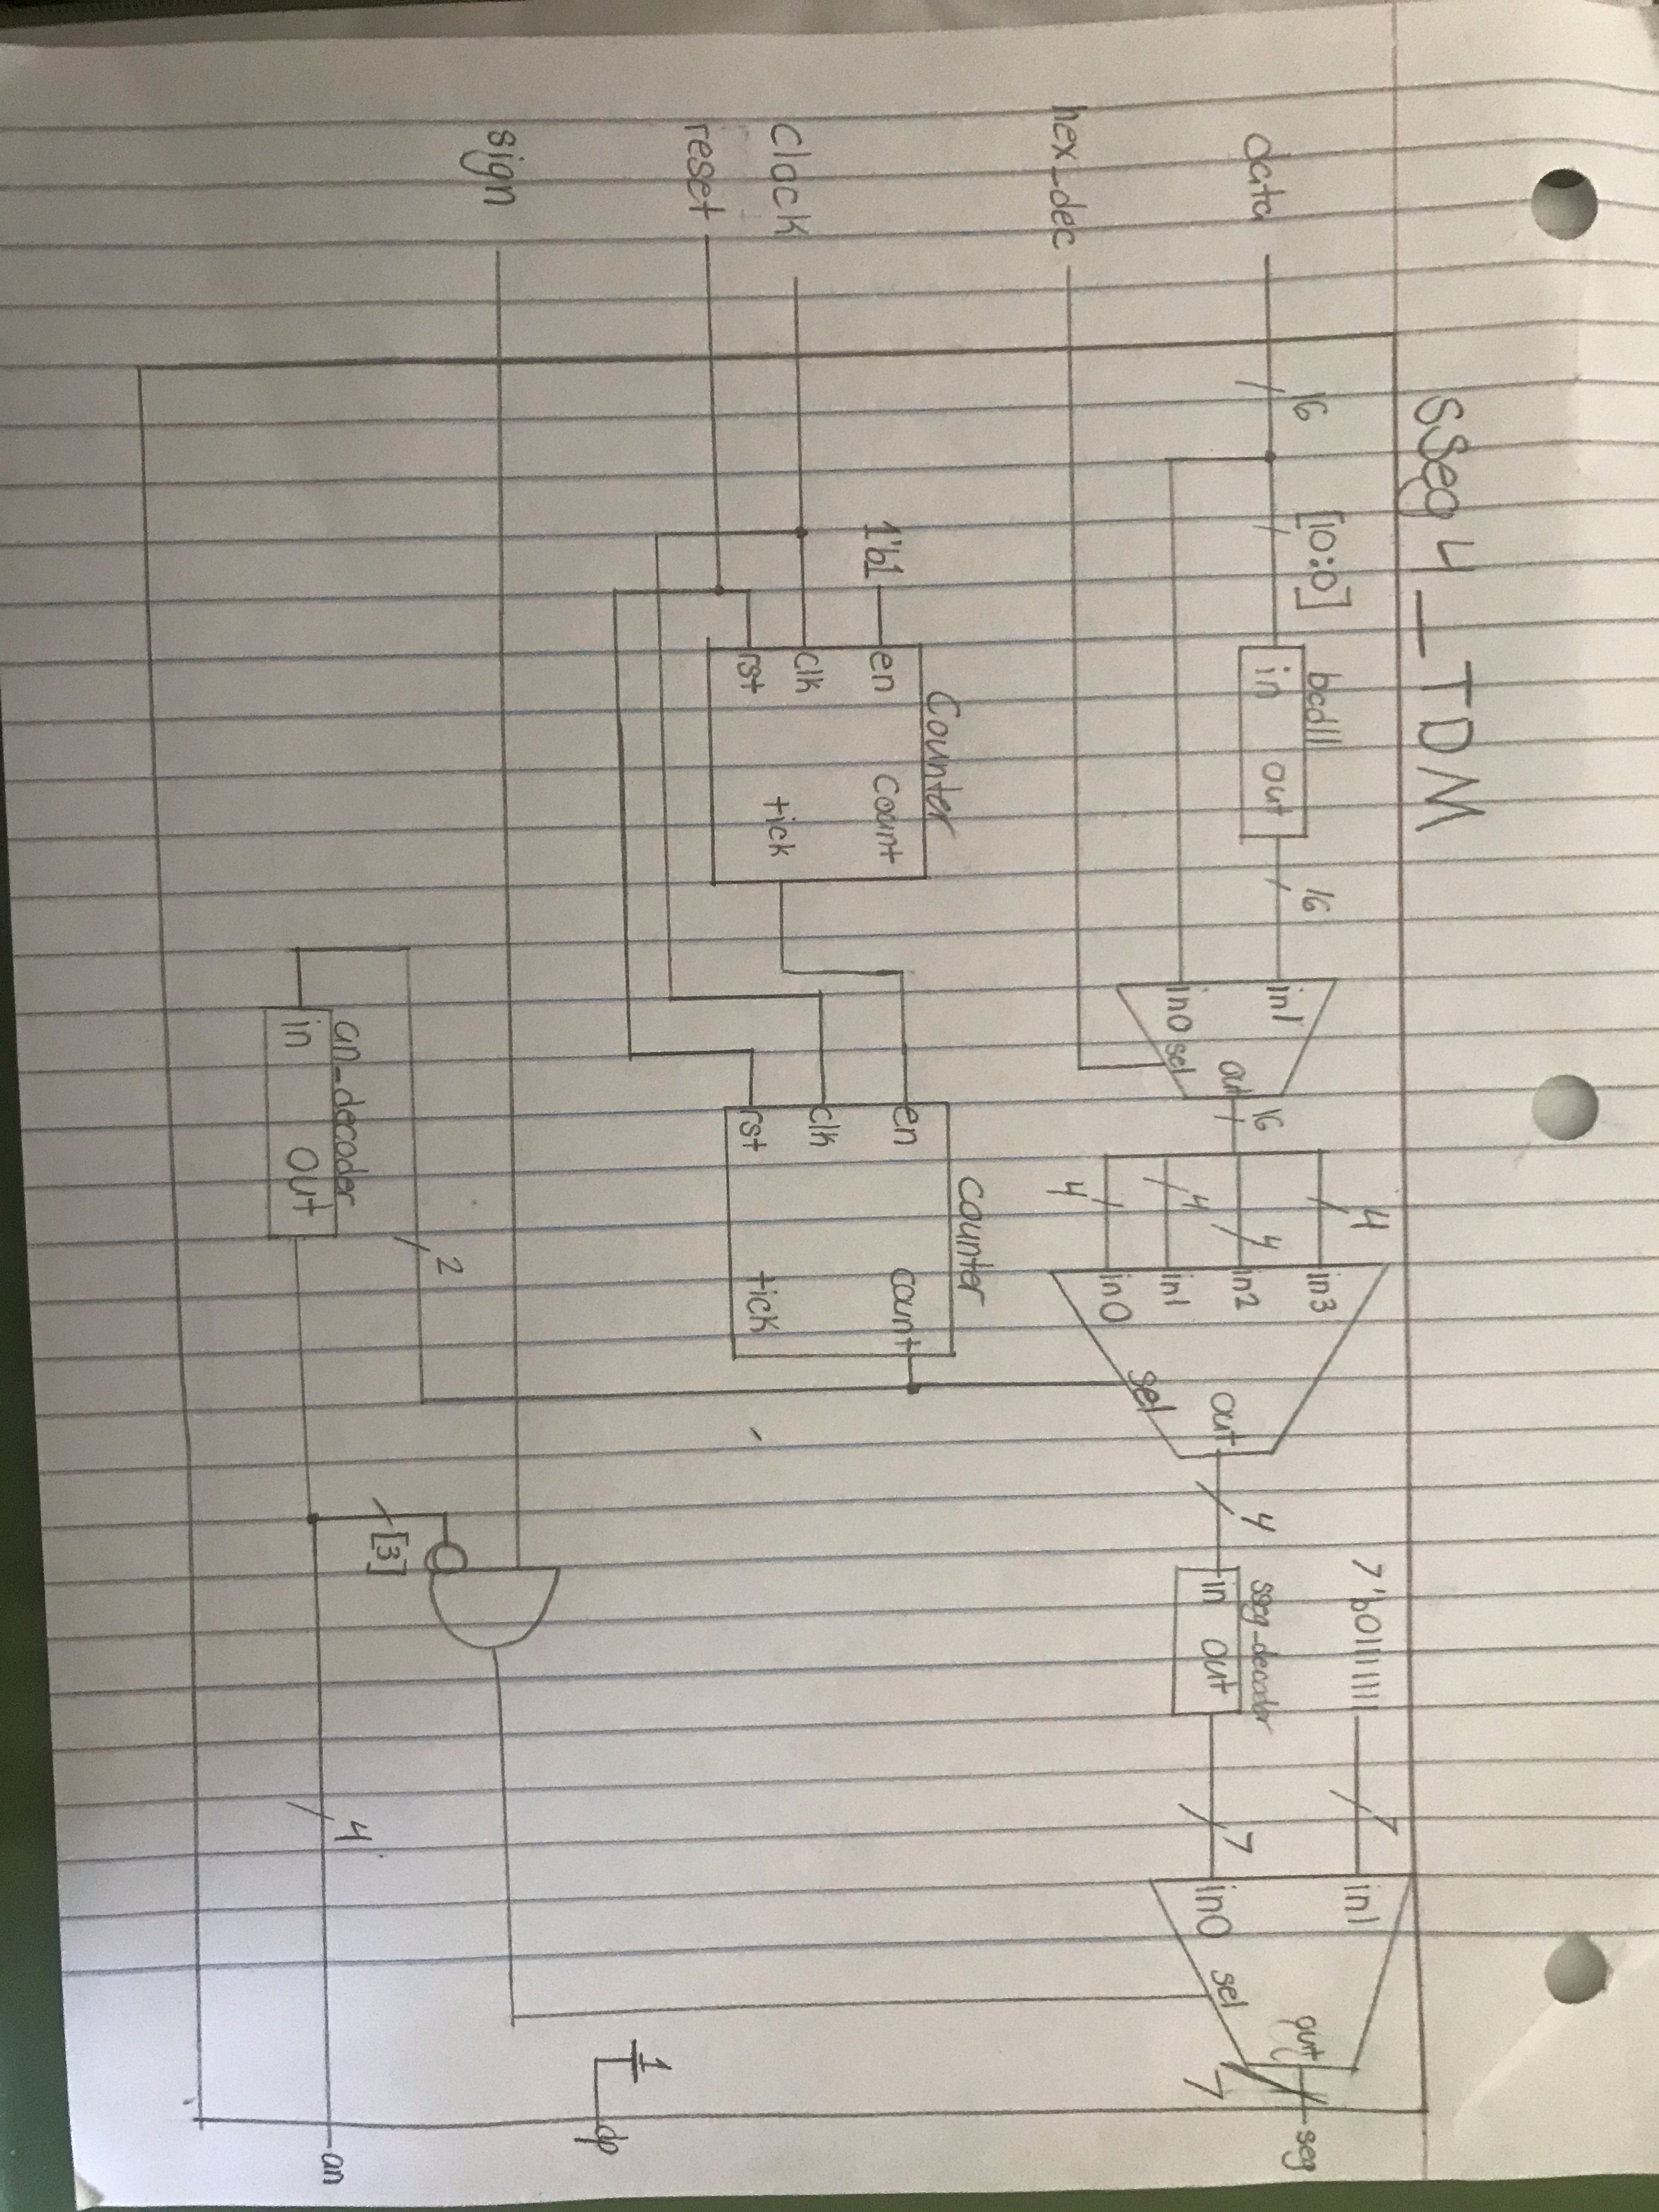
\includegraphics[width=1.05\textwidth]{sseg4_TDM_Schematic.jpeg}
	\label{fig:picture}
\end{figure}

\begin{figure}[ht]\centering
	\caption{calclab10 Schematic}
%	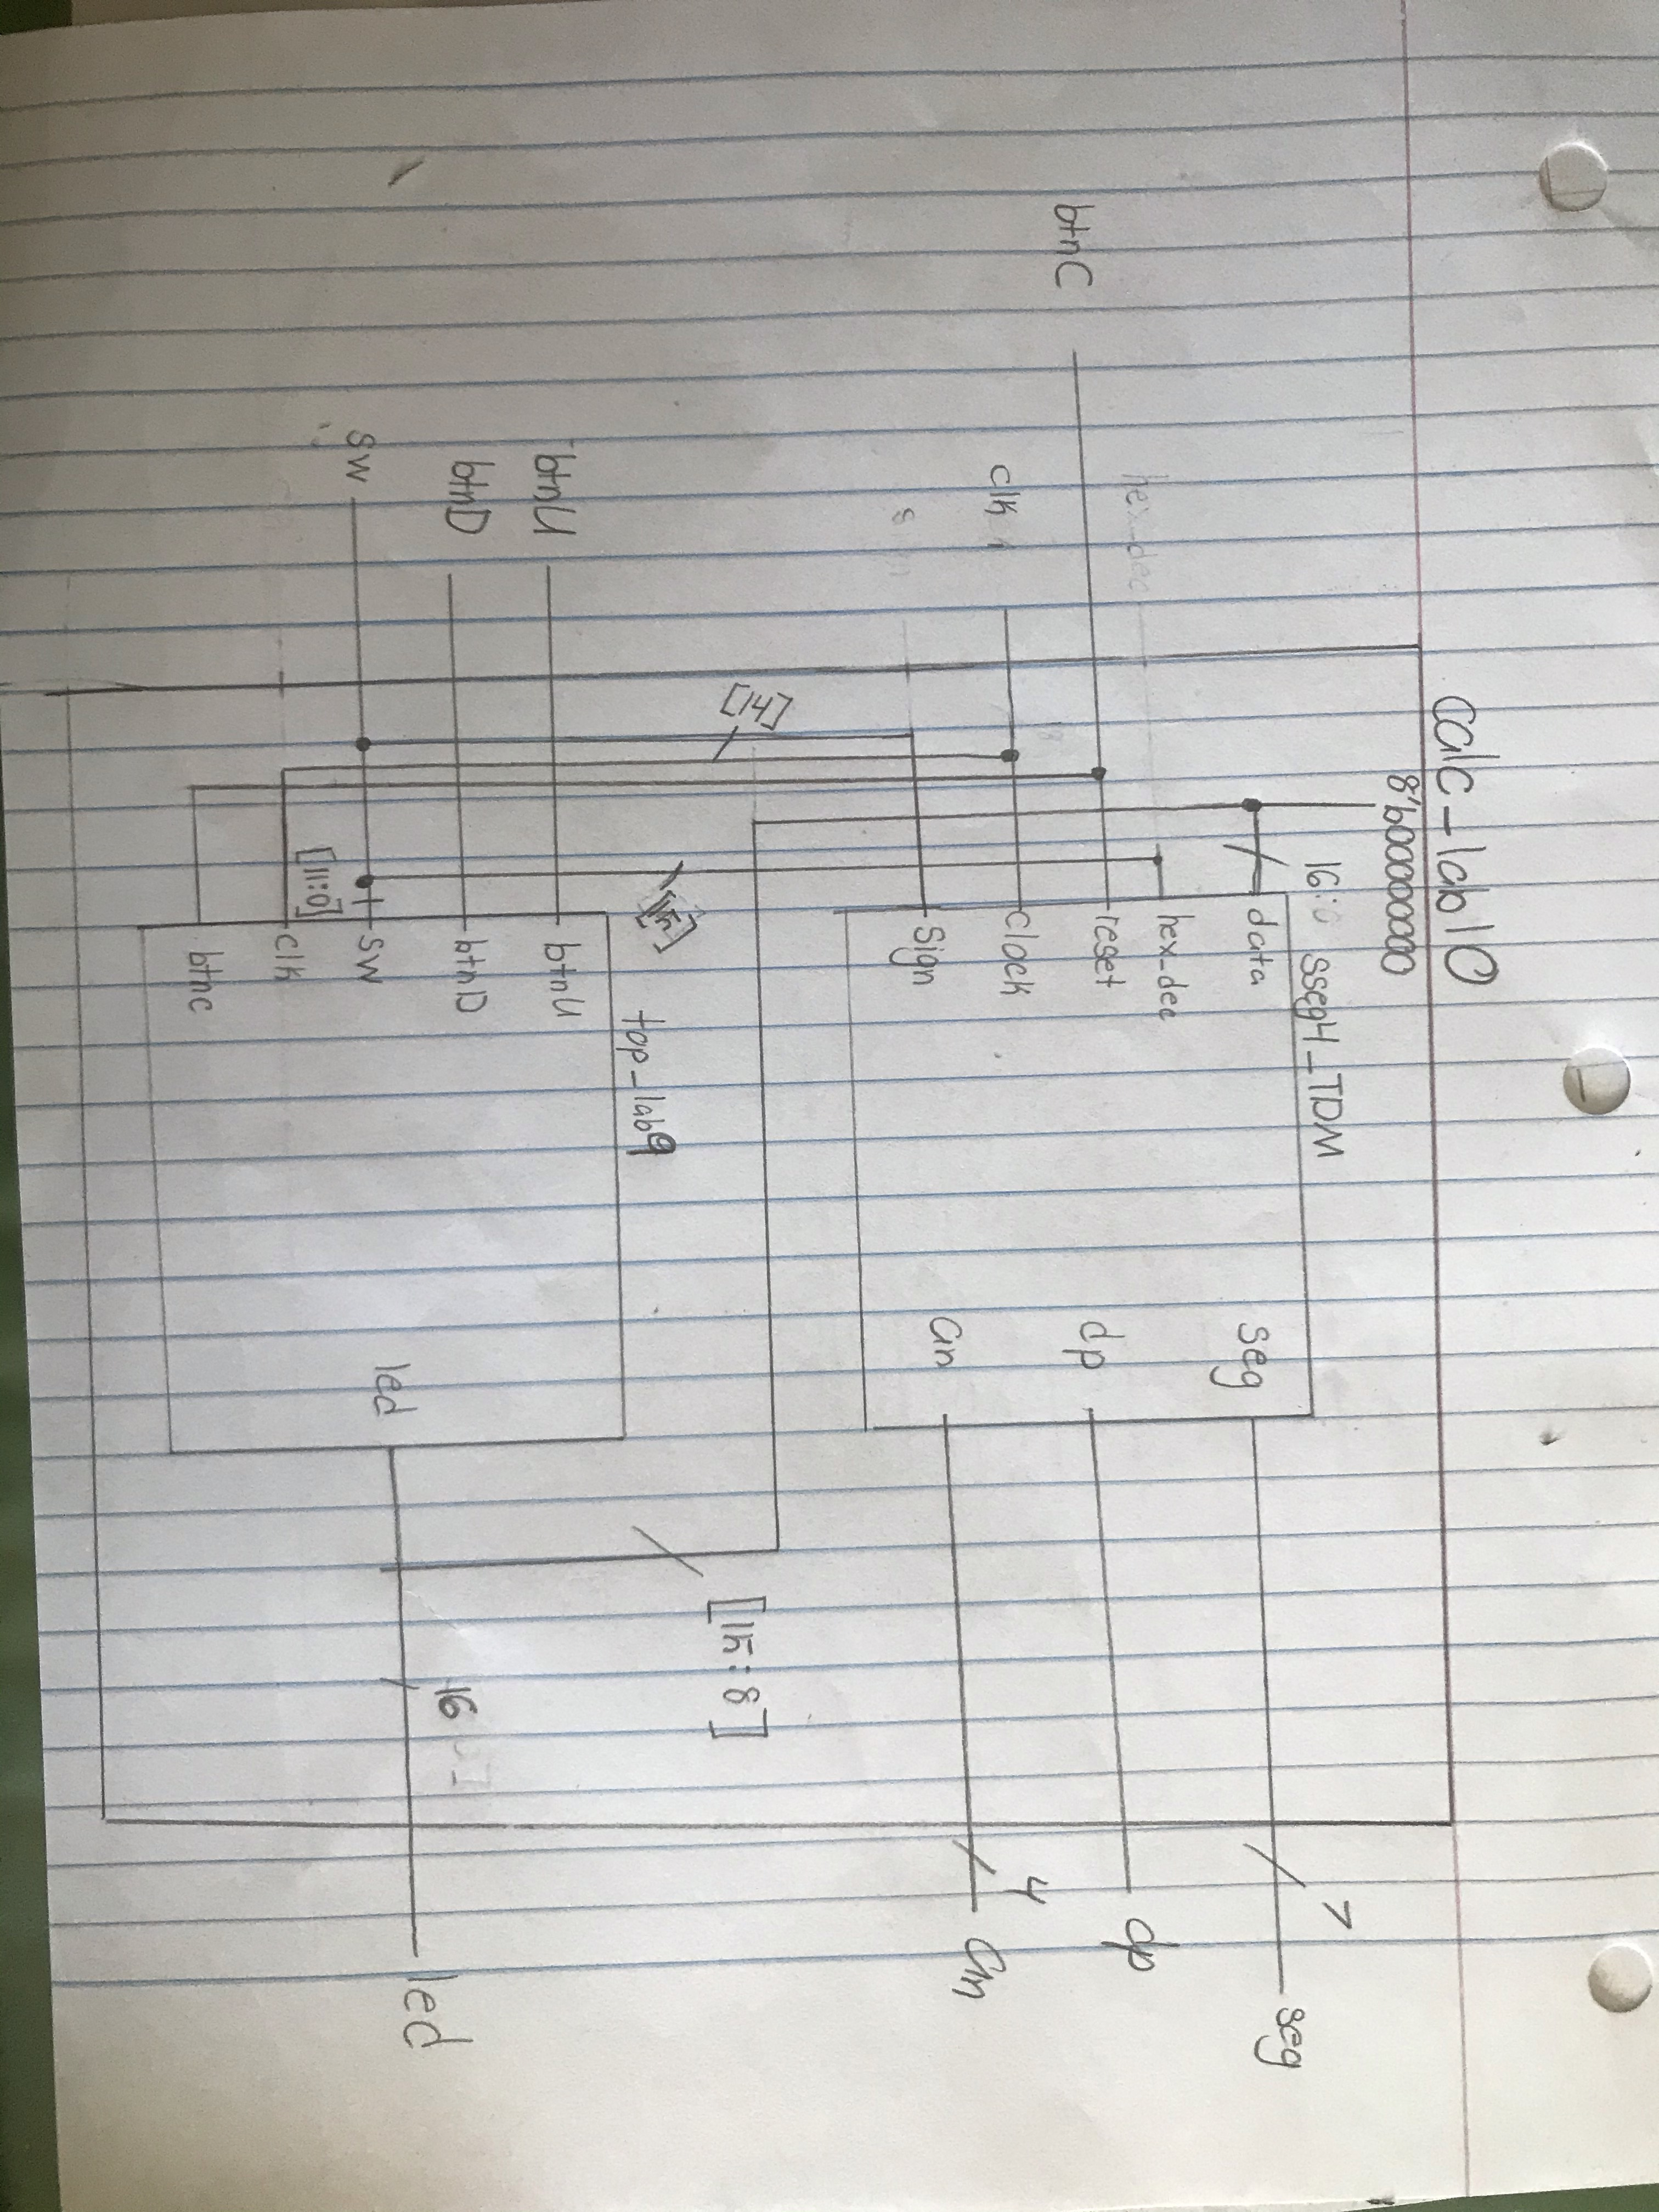
\includegraphics[width=1.15 \textwidth]{calc_lab10_Schematic.jpeg}
	\label{fig:picture}
\end{figure}

\clearpage
\section*{Code}

\begin{lstlisting}[style=Verilog,
caption=guess FSM Module,
label=guess FSM 
]

`timescale 1ns / 1ps
//ELC 2137, Jake Simmons, 2020-04-20

module guess_FSM (
	input [3:0]b,
	input reset,
	input clk,
	output reg [3:0]y,
	output reg win,
	output reg lose
	);

	//states
	localparam [2:0]
		S0 = 3'b000,
		S1 = 3'b001,
		S2 = 3'b010,
		S3 = 3'b011,
		SWIN = 3'b100,
		SLOSE = 3'b101;

	//internal signals
	reg[2:0] nState, State;

	always_ff @(posedge clk or posedge reset)
		if(reset == 1) begin
			State <= S0;
		end
		else begin
			State <= nState;
		end


	always_comb begin
		case(State)
		S0: begin
			y[0] = 1;
			y[3:1] = 0;
			lose = 1'b0;
			win = 1'b0;
			if(b==1)
				nState = SWIN;
			else if(b==0)
				nState = S1;
			else 
				nState = SLOSE;
			end

		S1: begin
			y[1] = 1;
			y[0] = 0;
			y[3:2] = 0;
			if(b==2)
				nState = SWIN;
			else if(b==0)
				nState = S2;
			else 
				nState = SLOSE;
			end

		S2: begin
			y[2] = 1;
			y[3] = 0;
			y[1:0] = 0;
			if(b==4)
				nState = SWIN;
			else if(b==0)
				nState = S3;
			else 
				nState = SLOSE;
			end

			S3: begin
				y[3] = 1;
				y[2:0] = 0;
				if(b==8)
					nState = SWIN;
				else if(b==0)
					nState = S0;
				else 
					nState = SLOSE;
				end

				SWIN: begin
					win = 1'b1;
					lose = 1'b0;
					if(b==0)
						nState = S0;
					else
						nState = SWIN;
					end

				SLOSE: begin
					lose = 1'b1;
					win = 1'b0;
					if(b==0)
						nState = S0;
					else
						nState = SLOSE;
					end
				endcase
			end   
endmodule
\end{lstlisting}


\begin{lstlisting}[style=Verilog,
caption=guess FSM Test Bench,
label=guess_FSM_test
]
`timescale 1ns / 1 ps
//ELC 2137, Jake Simmons, 2020-04-21
module guess_FSM_test();

	reg clk, reset;
	reg [3:0] b;
	wire [3:0] y;
	wire win, lose;

	guess_FSM gs( .clk(clk), .b(b), .reset(reset), .y(y), .win(win),
	.lose(lose) );

	always begin
		clk = ~clk; #10;
	end

	initial begin
		clk = 0; reset = 0; b = 0; #10;
		reset = 1; #10;
		reset = 0; #10;

		b = 0; #10; //S1
		b = 0; #10; //S2
		b = 0; #10; //S3

		b = 0; #10; //S0
		b = 1; #20; //SWIN
		b = 2; #10; //SWIN

		b = 0; #10 //S0;
		b = 2; #10; //SLOSE
		b = 1; #10; //SLOSE

		b = 0; #10; //S0
		b = 0; #10; //S1
		b = 2; #10; //SWIN
		b = 2; #10; //SWIN

		b = 0; #10; //S0
		b = 0; #10; //S1
		b = 1; #10; //SLOSE
		b = 1; #10; //SLOSE

		b = 0; #10; //S0
		b = 0; #10; //S1
		b = 0; #10; //S2
		b = 4; #10; //SWIN
		b = 2; #10; //SWIN
		b = 0; #10; //S0
		b = 0; #10; //S1
		b = 0; #10; //S2
		b = 1; #10; //SLOSE
		b = 1; #10; //SLOSE
		b = 0; #10; //S0

		b = 0; #10; //S1
		b = 0; #10; //S2
		b = 0; #10; //S3
		b = 8; #10; //SWIN
		b = 2; #10; //SWIN
		b = 0; #10; //S0
		b = 0; #10; //S1
		b = 0; #10; //S2
		b = 0; #10; //S3
		b = 1; #10; //SLOSE
		b = 1; #10; //SLOSE
		b = 0; #10; //S0


	end
endmodule

\end{lstlisting}

\begin{lstlisting}[style=Verilog,
caption=guessing game Module,
label=game
]
`timescale 1ns / 1ps
// ELC 2137, Jake Simmons, 2020-04-22

module guessing_game(
	input btnU,
	input btnD,
	input btnR,
	input btnL,
	input btnC,
	input clk,
	input [15:0]sw,
	output [6:0] seg,
	output [3:0] an,
	output [15:0] led,
	output dp
	);

	wire [3:0] W1;
	wire [1:0] W2;
	wire [15:0] W3;
	wire [3:0] W4;
	wire W5, W6;
	wire [1:0] W7;

	debounce #(.N(21)) d1( .in(btnU), .clk(clk), .reset(btnC), .out(W1[3]));
	debounce #(.N(21)) d2( .in(btnR), .clk(clk), .reset(btnC), .out(W1[2]));
	debounce #(.N(21)) d3( .in(btnD), .clk(clk), .reset(btnC), .out(W1[1]));
	debounce #(.N(21)) d4( .in(btnL), .clk(clk), .reset(btnC), .out(W1[0]));

	Counter #(.N(25)) count( .clk(clk), .en(1'b1), .tick(W2));
	Counter #(.N(23)) count1( .clk(clk), .en(1'b1), .tick(W7));

	mux2 #(.N(25)) m( .in1(W2), .in0(W7), .sel(sw[0]), .out(W3));

	guess_FSM gFSM( .b(W1), .clk(W3), .y(W4), .win(W5), .lose(W6), .reset(btnC));

	//top
	assign seg[0] = ~W4[3];

	//right
	assign seg[1] = ~W4[2];

	assign seg[4:2] = 3'b111;

	//left
	assign seg[5] = ~W4[0];

	//bottom
	assign seg[6] = ~W4[1];

	//win
	assign led[0] = W5;

	//lose
	assign led[1] = W6;


	assign led[15:2] = 14'b00000000000000;
	assign an = 4'b1110;

	assign dp = 1'b1;

	endmodule



\end{lstlisting}

\begin{lstlisting}[style=Verilog,
caption=sseg4TDM Test Bench,
label=sseg4TDM Test
]
`timescale 1ns / 1ps
//ELC 2137 2020-7-4

module sseg4_TDM_test();
	reg clock;
	reg reset;
	reg [15:0] data;
	reg hex_dec;
	reg sign;
	wire [6:0] seg;
	wire dp;
	wire [3:0] an;

	sseg4_TDM sseg4( .clock(clock), .reset(reset), .data(data), .hex_dec(hex_dec),
	.sign(sign), .seg(seg), .dp(dp), .an(an));



	// clock runs continuously 

	always begin 

		clock = ~clock; #10; 

	end

	// this block only runs once 

	initial begin
		data = 0; hex_dec = 0; reset = 1;  clock = 0; sign = 0; #2621440;
		data = 1; hex_dec = 1; reset = 0;  sign = 0; #2621440;
		data = 2; hex_dec = 1; reset = 0;  sign = 0;  #2621440;
		data = 3; hex_dec = 1; reset = 0;  sign = 0;  #2621440;
		data = 4; hex_dec = 1; reset = 0;  sign = 0;  #2621440;
		data = 5; hex_dec = 1; reset = 0;  sign = 0;  #2621440;
		data = 6; hex_dec = 1; reset = 0;  sign = 0;  #2621440;
		data = 7; hex_dec = 1; reset = 0;  sign = 0;  #2621440;
		data = 8; hex_dec = 0; reset = 0;  sign = 1;  #2621440;
		data = 9; hex_dec = 0; reset = 0;  sign = 1;  #2621440;
		data = 10; hex_dec = 0; reset = 0;  sign = 1;  #2621440;
		data = 11; hex_dec = 0; reset = 0;  sign = 1;  #2621440;
		data = 12; hex_dec = 1; reset = 0;  sign = 1;  #2621440;
		data = 13; hex_dec = 1; reset = 0;  sign = 1;  #2621440;
		data = 14; hex_dec = 0; reset = 0;  sign = 0;  #2621440;
		data = 15; hex_dec = 0; reset = 0;  sign = 0;  #2621440;

	$finish;

	end
endmodule


\end{lstlisting}

\begin{lstlisting}[style=Verilog,
caption=calclab10 Module,
label=calclab10
]

`timescale 1ns / 1ps
//ELC 2137 Jake Simmons 2020-4-8

module calc_lab10(
	input clk,
	input btnU,
	input btnD,
	input [11:0] sw,
	input btnC,
	output [15:0] led,
	output [6:0] seg,
	output dp,
	output [3:0] an
	);
	wire [7:0] W1;

	sseg4_TDM disp_unit( .data({8'b00000000, W1}), .hex_dec(sw[15]),
	.reset(btnC), .clock(clock), .sign(sw[14]), 
	.seg(seg), .dp(dp), .an(an));

	top_lab9 calc_unit( .btnU(btnU), .btnD(btnD), .sw(sw[11:0]),
	.clk(clk), .btnC(btnC), .led(led) );

	assign w1 = led[15:8];
endmodule


\end{lstlisting}


\end{document}
